\documentclass{report}
\usepackage[T1]{fontenc}
\usepackage[utf8]{inputenc} % if using pdflatex
\usepackage{csquotes}
\usepackage{float}
\usepackage{graphicx}
\usepackage{amsmath}
\usepackage{amsfonts}
\usepackage[italian]{babel}
\usepackage[a4paper,margin=2.5cm]{geometry}
\usepackage[]{hyperref}
\usepackage{multicol}
\hypersetup{
    colorlinks=true,
    linkcolor=blue,
    filecolor=magenta,
    citecolor = blue,
    urlcolor=blue,
    pdftitle={Overleaf Example},
    pdfpagemode=FullScreen,
    }
\usepackage[
backend=bibtex,
style=ieee,
sorting=none,
]{biblatex}
\usepackage{xcolor}
\usepackage{listings}

\definecolor{codebg}{RGB}{245,245,244}
\definecolor{codegray}{RGB}{110,110,110}
\definecolor{codegreen}{RGB}{0,120,0}
\definecolor{codeblue}{RGB}{0,0,180}
\definecolor{codeorange}{RGB}{180,90,0}

\definecolor{codegreen}{rgb}{0,0.6,0}
\definecolor{codegray}{rgb}{0.5,0.5,0.5}
\definecolor{codepurple}{rgb}{0.58,0,0.82}
\definecolor{backcolour}{rgb}{0.95,0.95, 0.92}

\lstdefinestyle{Java}{
    language=Java,
    backgroundcolor=\color{codebg},
    basicstyle=\ttfamily\small,
    keywordstyle=\color{codeblue}\bfseries,
    commentstyle=\color{codegreen}\itshape,
    stringstyle=\color{codeorange},
    numberstyle=\tiny \color{black},
    numbers=left,
    stepnumber=1,
    numbersep=10pt,
    frame=single,
    rulecolor=\color{black!20},
    tabsize=4,
    showspaces=false,
    showstringspaces=false,
    breaklines=true,
    breakatwhitespace=true,
    columns=fullflexible,
    keepspaces=true,
    captionpos=b
}

\title{Report secondo progetto di Metodi del calcolo scientifico}
\author{Daniele Besozzi 894998 \\ Andrea Consonni 900116 \\ Matteo Cervini 902225}
\date{\today}

\addbibresource{bibliography.bib}

% TODOs:
% - Mettere snippet di codice generazione matrici in 1.1 dopo refactoring

\begin{document}
    \maketitle

    \tableofcontents
    \chapter{Prima parte: implementazione e benchmark DCT2}
    Per l'implementazione della DCT2 abbiamo scelto il linguaggio 
di programmazione Java, mettendo a confronto la nostra implementazione con
l'implementazione fornita dalla libreria \texttt{JTransform} \cite{wendykier_jtransforms_3_1}.
Per effettuare le operazioni di algebra lineare richieste in modo semplice ed ottimale, abbiamo
scelto di utilizzare la libreria \texttt{Efficient Java Matrix Library}(ejml)\cite{abeles_ejml_0_44_0}.
\section{Misurazione delle performance}
Per misurare le performance della nostra implementazione rispetto a quella della libreria, 
abbiamo generato in maniera causale matrici di dimensioni pari a $2^i, i = 3,\dots,12$.


    \chapter{Seconda parte: compressione immagini}
    \section{Test su immagini}
Per provare la nostra implementazione della compressione tramite DCT2, abbiamo scelto due immagini: una di Tony Pitony e una di Lena (immagine classica per l'image processing).
Per entrambe le immagini, abbiamo applicato la DCT2 con diversi valori di $f$ (la dimensione del blocco) e $d$ (il numero di coefficienti da mantenere).
Di seguito sono riportati i risultati ottenuti per ciascuna immagine, le quali sono anche disponibili in formato \texttt{.bmp} al \href{https://drive.google.com/drive/folders/1BKgunC00Pi3_k0nMBObjdeB1KHGHyaLH}{link}.
\subsection{Tony Pitony}
Per quanto riguarda l'immagine in figura \ref{fig:tony_pitony} abbiamo provato a modificare la dimensione dei blocchi $f$ e il coefficiente del taglio $d$.
I valori di $f$ che abbiamo scelto sono stati $8$, $16$, $32$, $64$ e $128$, mentre i valori di $d$ sono stati rispettivamente $4$, $8$, $16$, $32$ e $64$, ovvero la metà della dimensione del blocco.
Fare benchmark aumentando la dimensione dei blocchi può risultare interessante per questa immagine perché contiene sia aree uniformi sia dettagli ad alta frequenza, come i bordi degli occhiali e la texture della camicia.
Blocchi più grandi migliorano generalmente la compressione nelle zone lisce, ma possono introdurre artefatti più evidenti e perdita di dettaglio nelle regioni ricche di dettagli.
\begin{figure}[H]
	\centering
	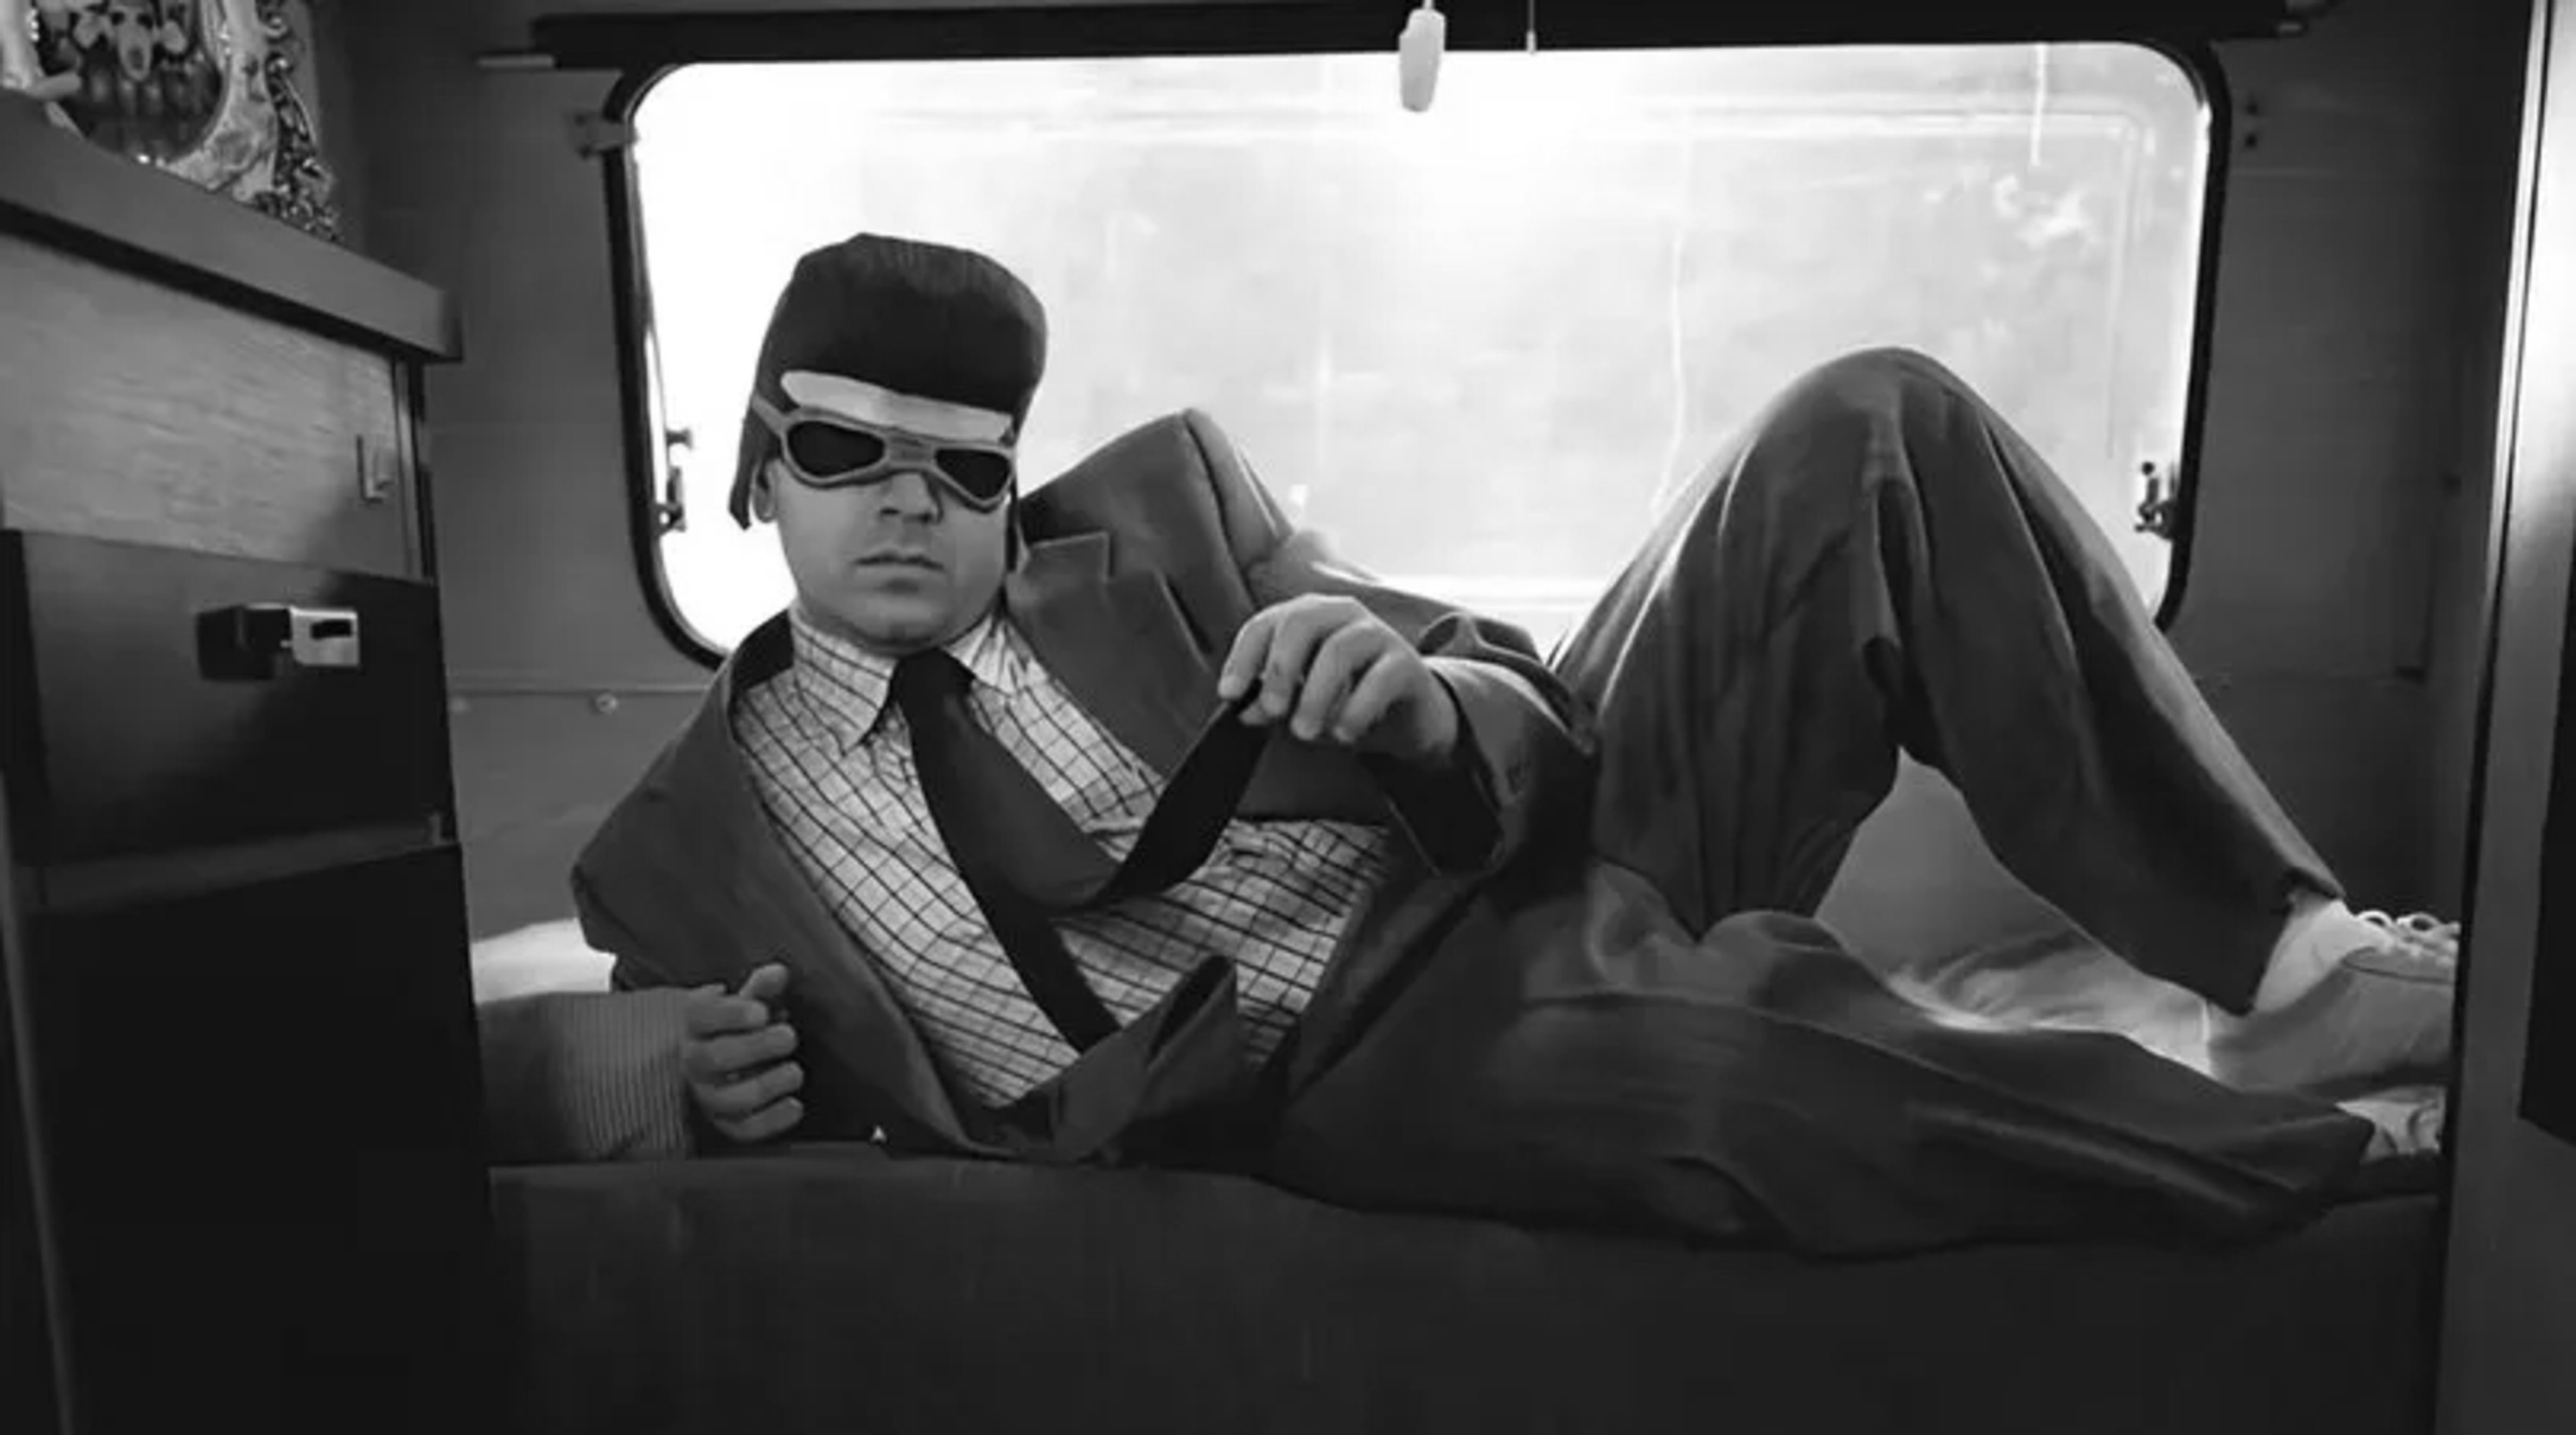
\includegraphics[width=0.8\textwidth]{figures/tonypitony.pdf}
	\caption{Immagine di Tony Pitony non compressa}
	\label{fig:tony_pitony}
\end{figure}
\begin{figure}[hbt]
	\centering
	% limit graphic size to avoid "Dimension too large" errors
	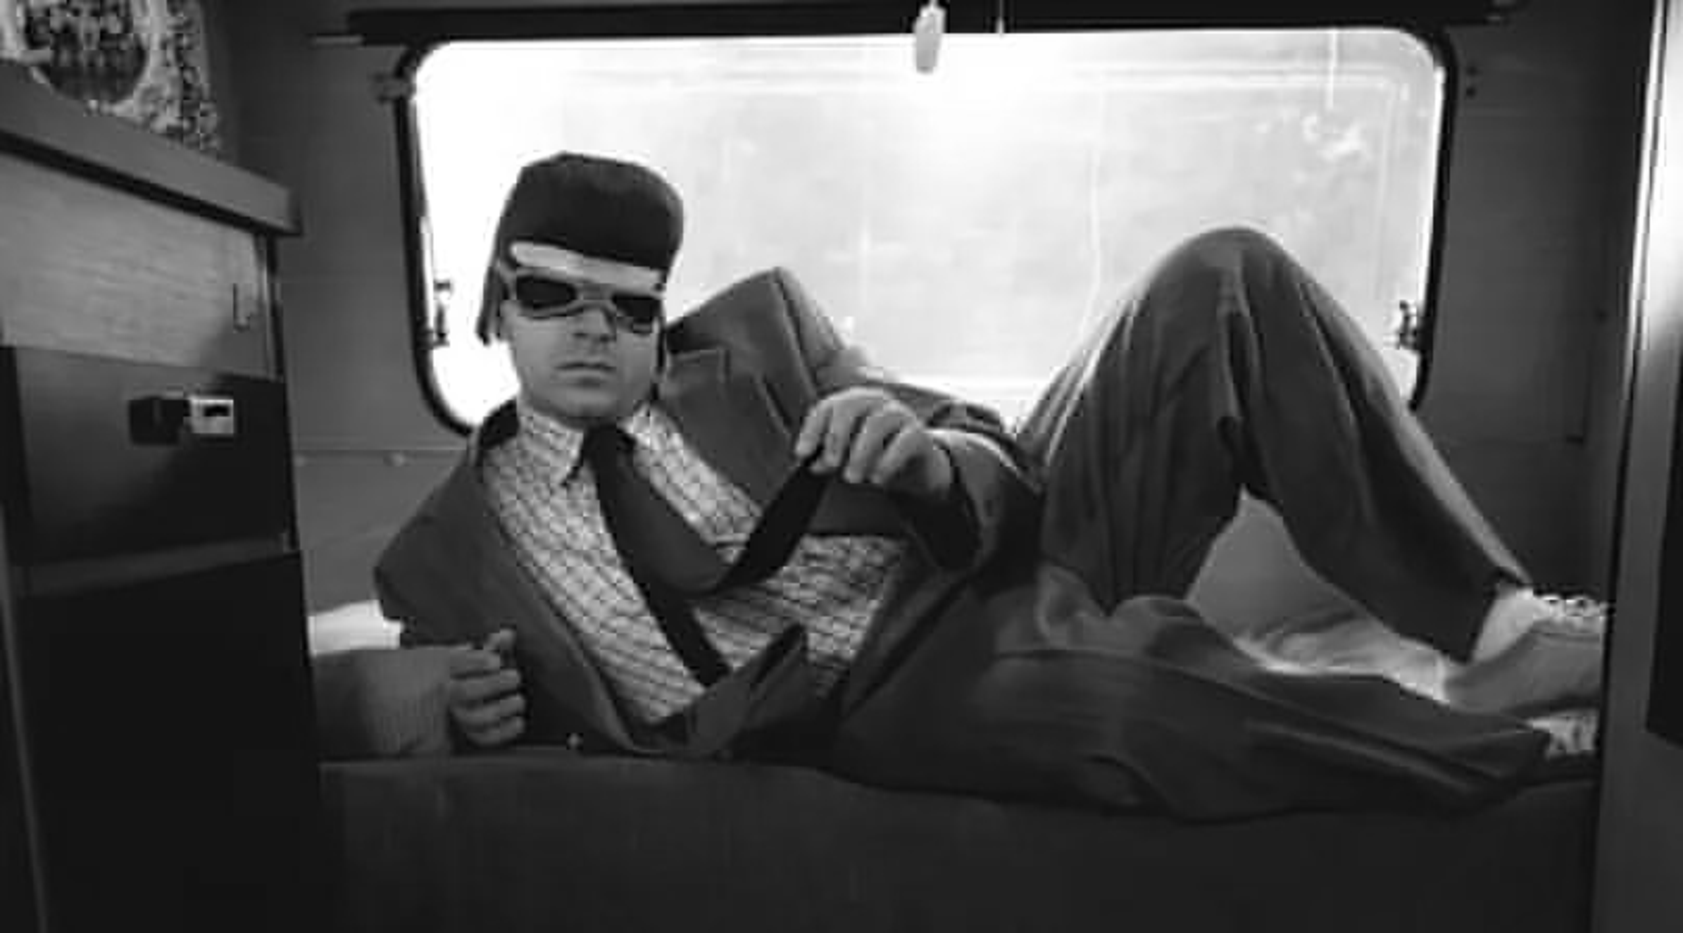
\includegraphics[width=0.8\textwidth]{figures/tonypitony_compressed_f8_d4.pdf}
	\caption{Immagine di Tony Pitony compressa con DCT2, con $f=8$ e $d=4$}
	\label{fig:tony_pitony_compressed_f8_d4}
\end{figure}
\begin{figure}[hbt]
	\centering
	% limit graphic size to avoid "Dimension too large" errors
	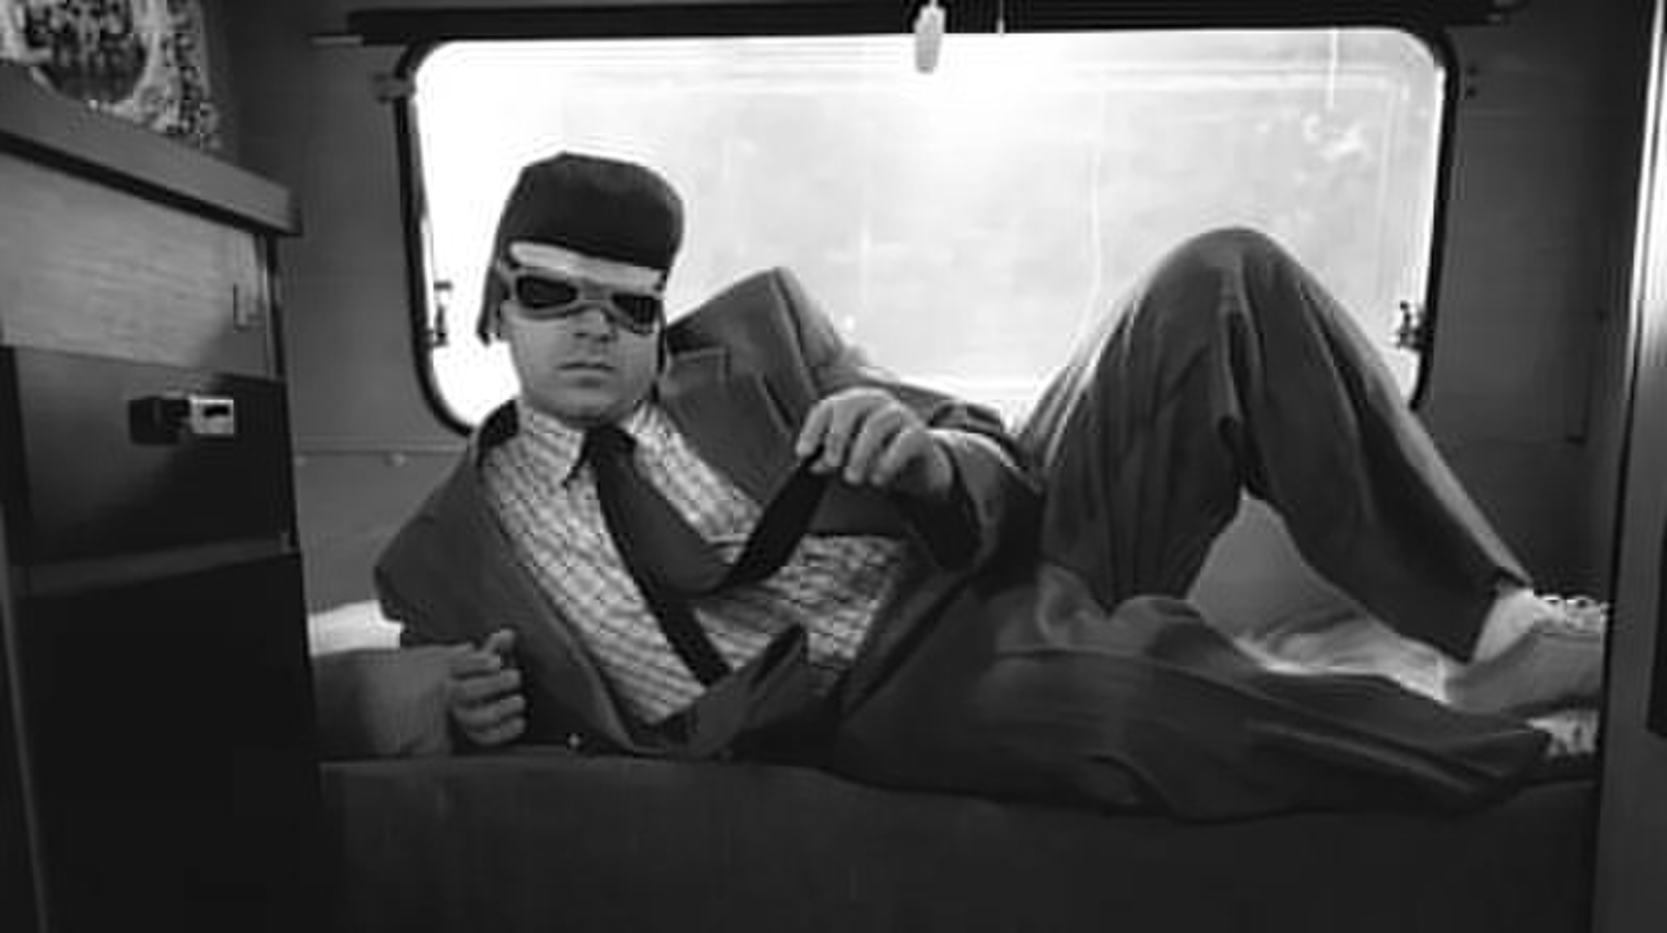
\includegraphics[width=0.8\textwidth]{figures/tonypitony_compressed_f16_d8.pdf}
	\caption{Immagine di Tony Pitony compressa con DCT2, con $f=16$ e $d=8$}
	\label{fig:tony_pitony_compressed_f16_d8}
\end{figure}
\begin{figure}[hbt]
	\centering
	% limit graphic size to avoid "Dimension too large" errors
	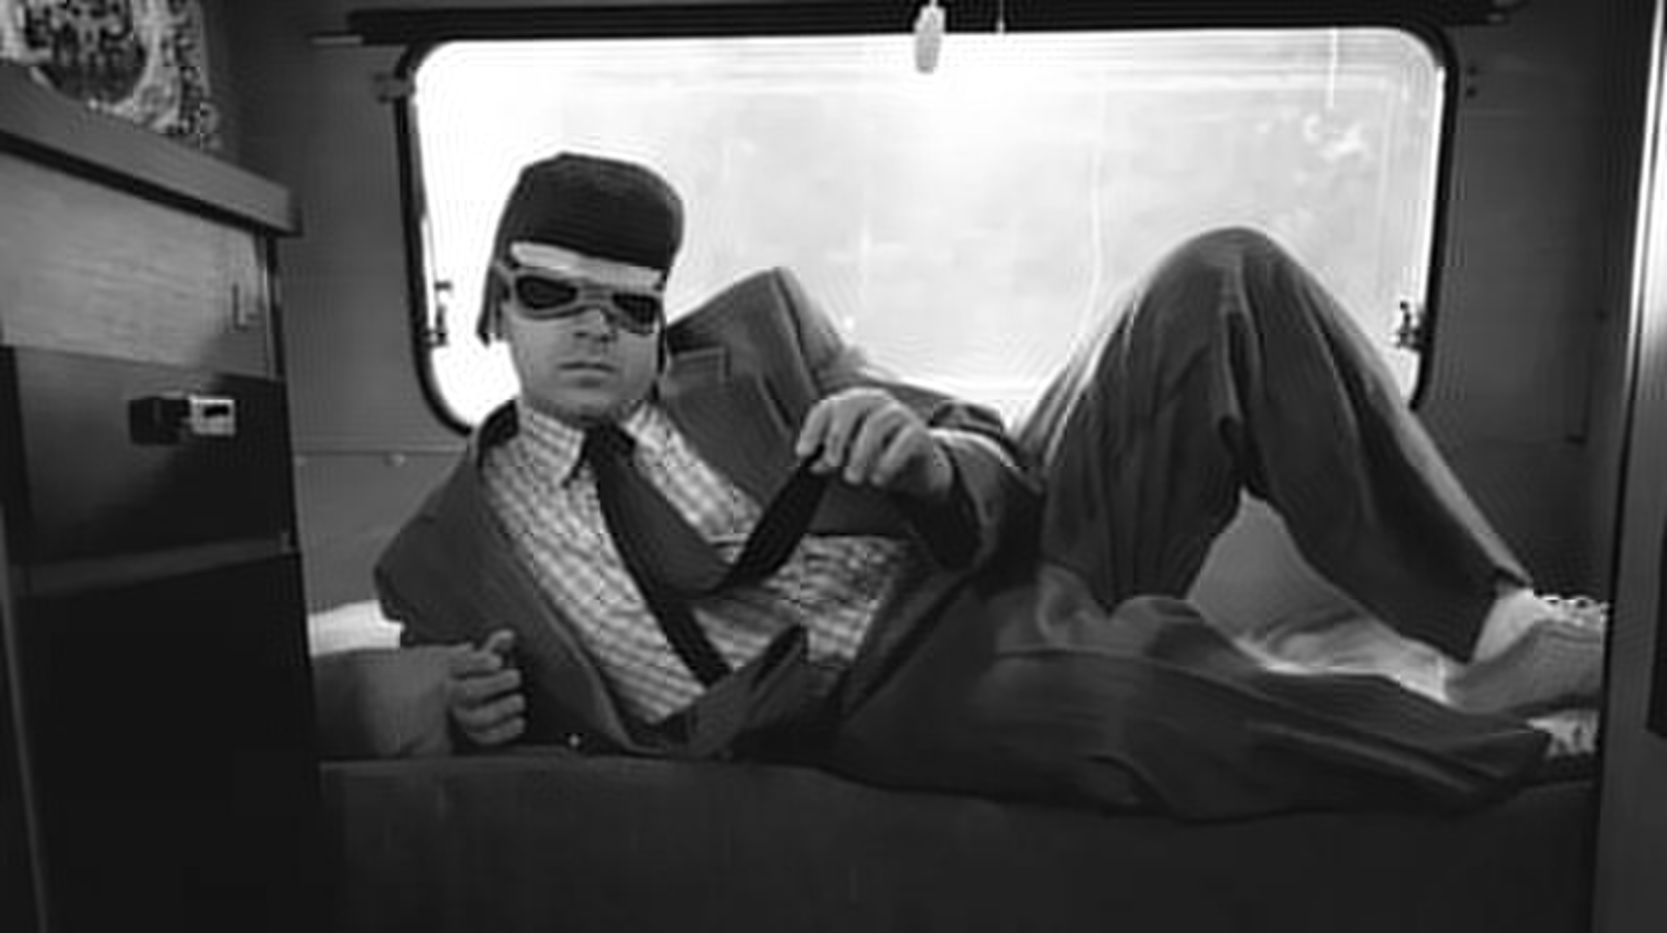
\includegraphics[width=0.8\textwidth]{figures/tonypitony_compressed_f32_d16.pdf}
	\caption{Immagine di Tony Pitony compressa con DCT2, con $f=32$ e $d=16$}
	\label{fig:tony_pitony_compressed_f32_d16}
\end{figure}

\begin{figure}[hbt]
	\centering
	% limit graphic size to avoid "Dimension too large" errors
	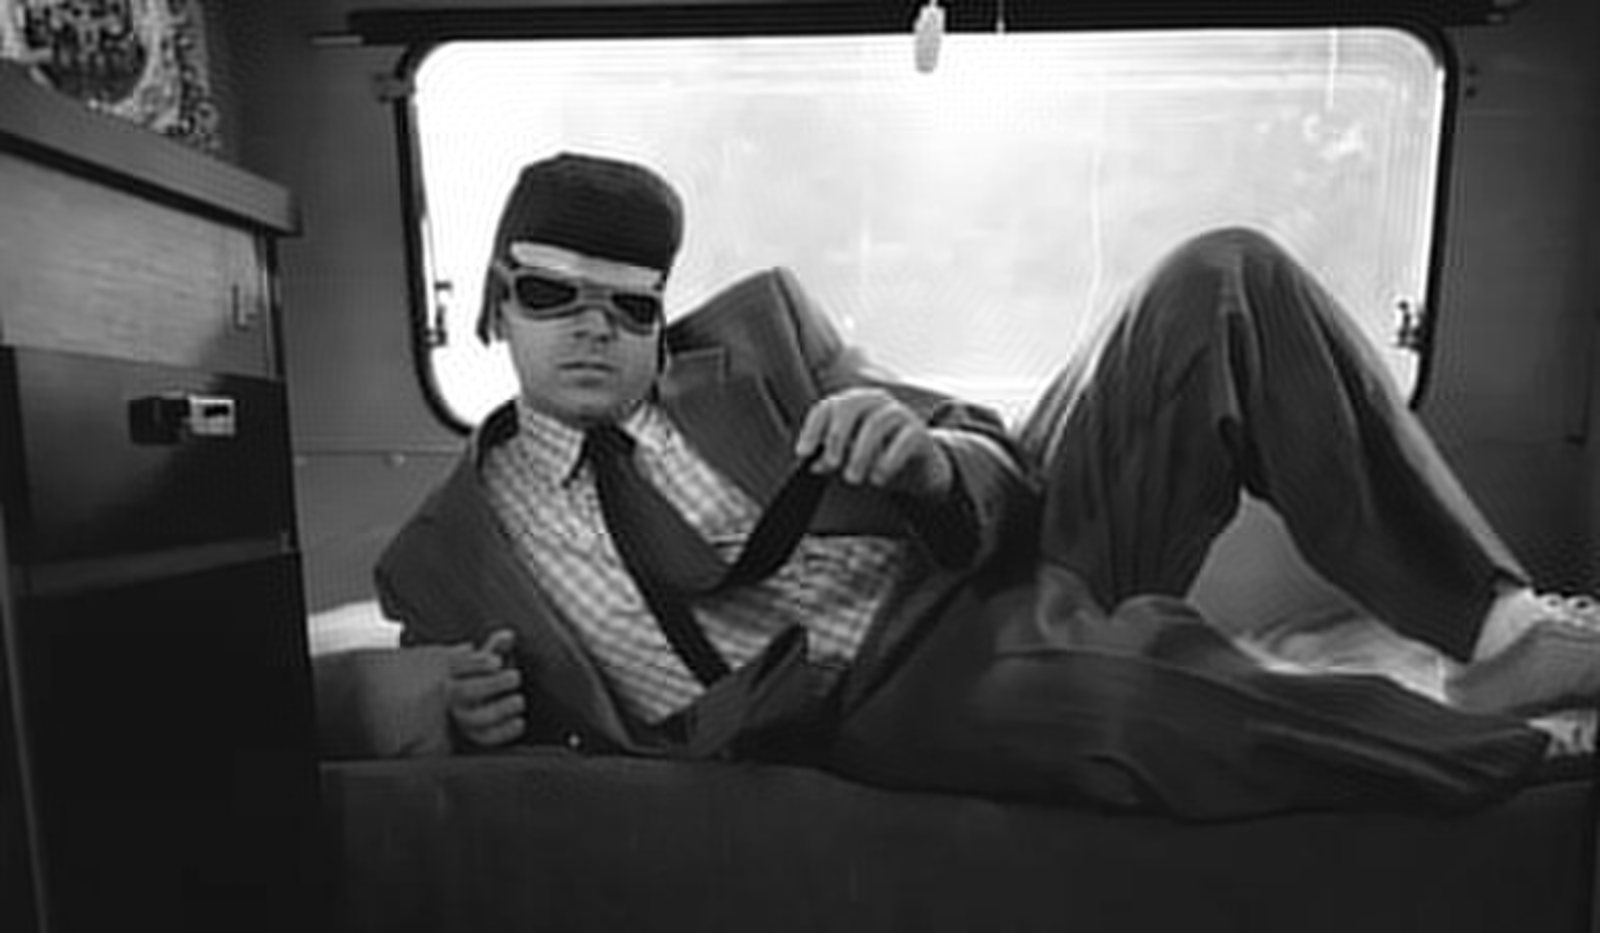
\includegraphics[width=0.8\textwidth]{figures/tonypitony_compressed_f64_d32.pdf}
	\caption{Immagine di Tony Pitony compressa con DCT2, con $f=64$ e $d=32$}
	\label{fig:tony_pitony_compressed_f64_d32}
\end{figure}
\begin{figure}[H]
	\centering
	% limit graphic size to avoid "Dimension too large" errors
	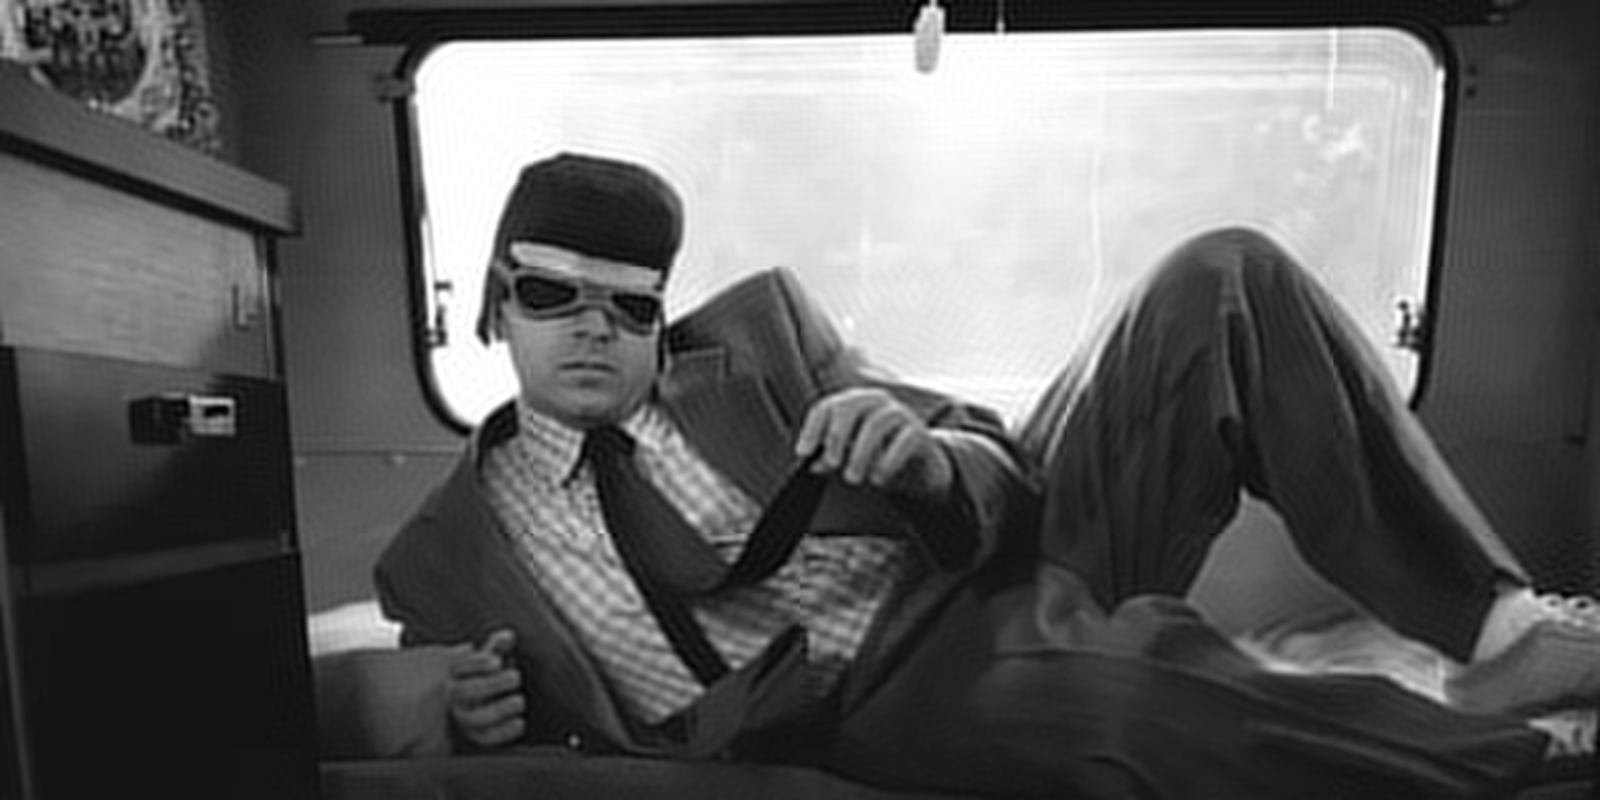
\includegraphics[width=0.8\textwidth]{figures/tonypitony_compressed_f128_d64.pdf}
	\caption{Immagine di Tony Pitony compressa con DCT2, con $f=128$ e $d=64$}
	\label{fig:tony_pitony_compressed_f128_d64}
\end{figure}
\noindent
All'aumentare della dimensione dei blocchi, possiamo vedere che la qualità dell'immagine compressa peggiora particolarmente nelle aree con molti dettagli. In particolare, si può anche notare l'introduzione di artefatti di tipo ringing nelle zone uniformi, come la finestra, che diventano più evidenti con blocchi più grandi.
Un esempio di questi artefatti è mostrato in figura \ref{fig:ringing}, dove si possono vedere delle bande scure e chiare intorno ai bordi, tipiche del fenomeno di ringing.
L'effetto sulle nostre immagini è evidenziato in figura \ref{fig:tony_pitony_ringing}, dove si possono notare le bande scure attorno alla gamba e ai bordi della finestra.
\begin{figure}[H]
	\centering
	% limit graphic size to avoid "Dimension too large" errors
	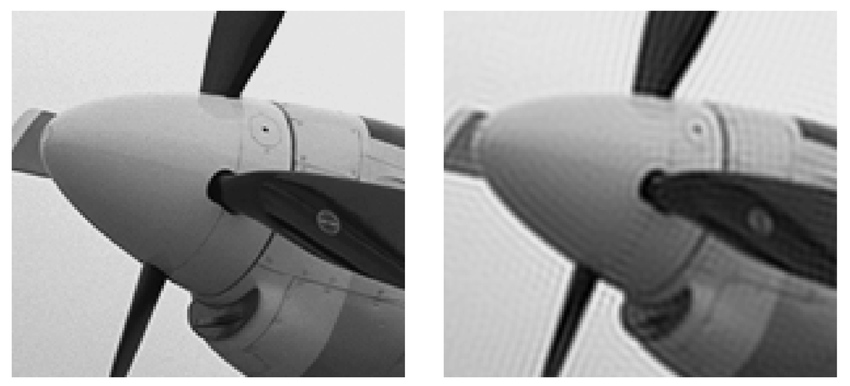
\includegraphics[width=0.8\textwidth]{figures/ringing.png}
	\caption{Artefatti di tipo ringing}
	\label{fig:ringing}
\end{figure}
\begin{figure}[H]
	\centering
	% limit graphic size to avoid "Dimension too large" errors
	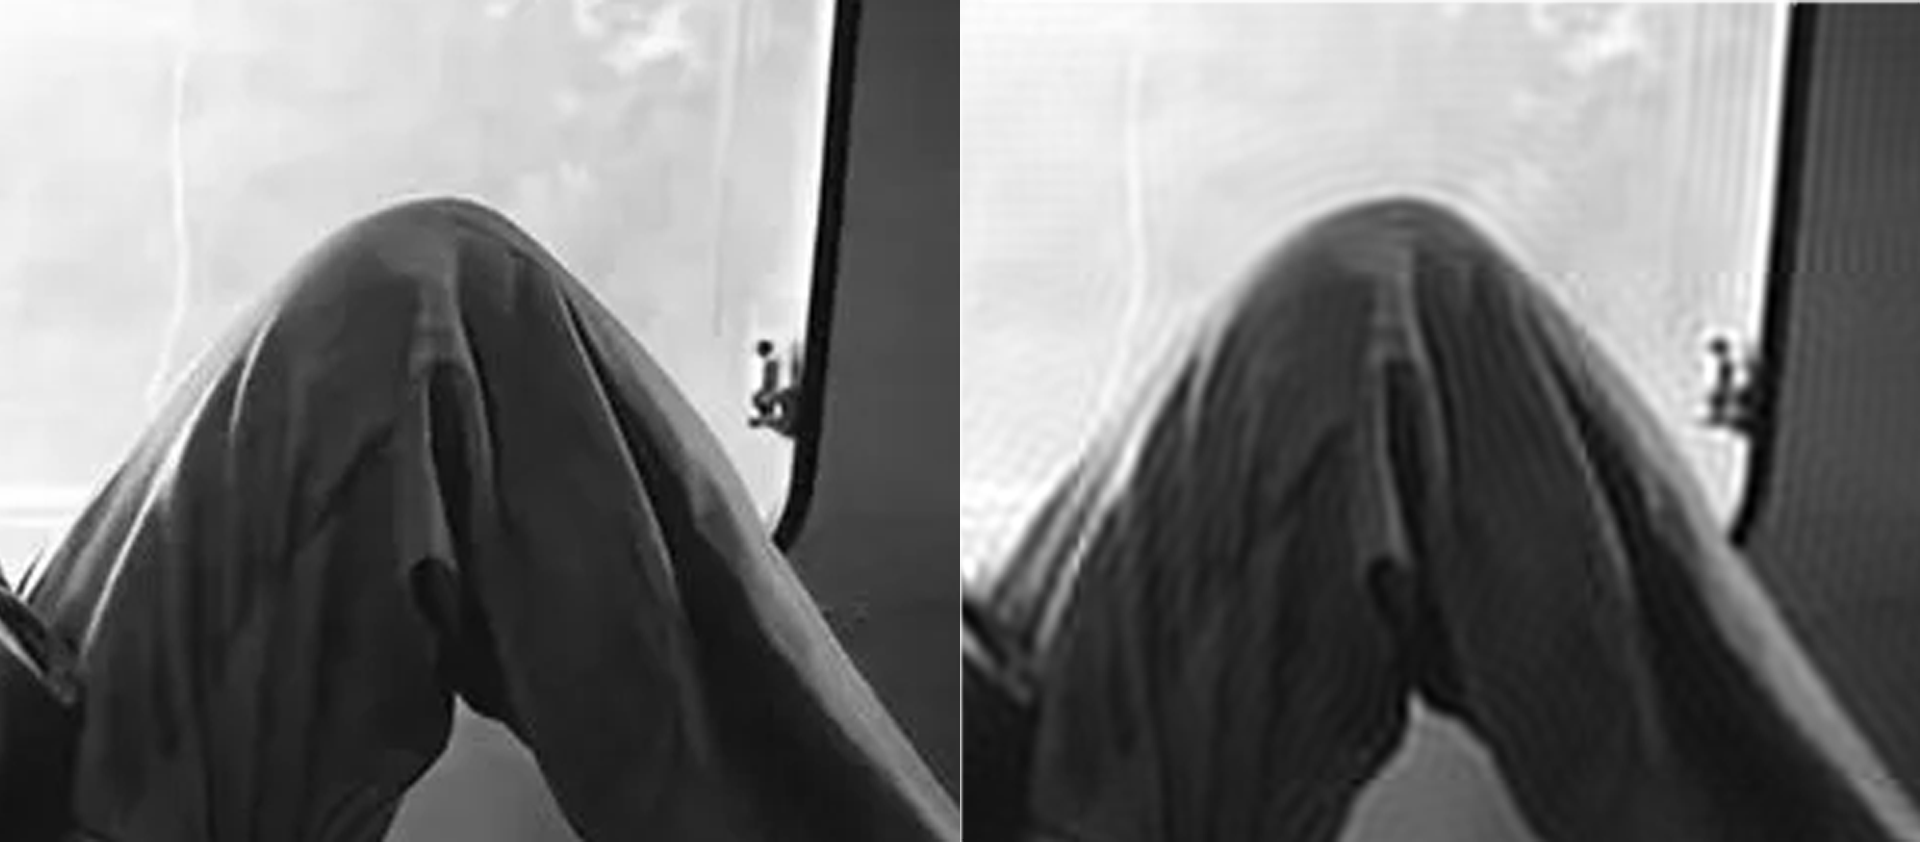
\includegraphics[width=0.8\textwidth]{figures/ringingTonyPitony.png}
	\caption{Zoom sull'immagine di Tony Pitony compressa con DCT2, con $f=128$ e $d=64$, evidenziando gli artefatti di tipo ringing}
	\label{fig:tony_pitony_ringing}
\end{figure}
\subsection{Lena}
Per quanto riguarda l'immagine in figura \ref{fig:lena} abbiamo provato a mantenere fissa la dimensione dei blocchi $f$ a $8$ e a modificare il coefficiente del taglio $d$ con i valori $12$, $8$, $4$, $2$ e $0$.
In particolare, con $d=0$ abbiamo eliminato tutti i coefficienti, ottenendo così un'immagine completamente nera.
Si può osservare che, come ci si aspetta, all'aumentare del numero di coefficienti mantenuti, la qualità dell'immagine compressa migliora, con una maggiore fedeltà all'immagine originale.
In particolare, con $d=12$ e $d=8$ l'immagine compressa è molto simile all'originale, mentre con $d=4$ si notano perdite di dettagli e si manifesta il tipico effetto di jpeg dove sono ben visibili i blocchi di dimensione $8\times8$.
\clearpage
\begin{multicols}{2}
\begin{figure}[H]
	\centering
	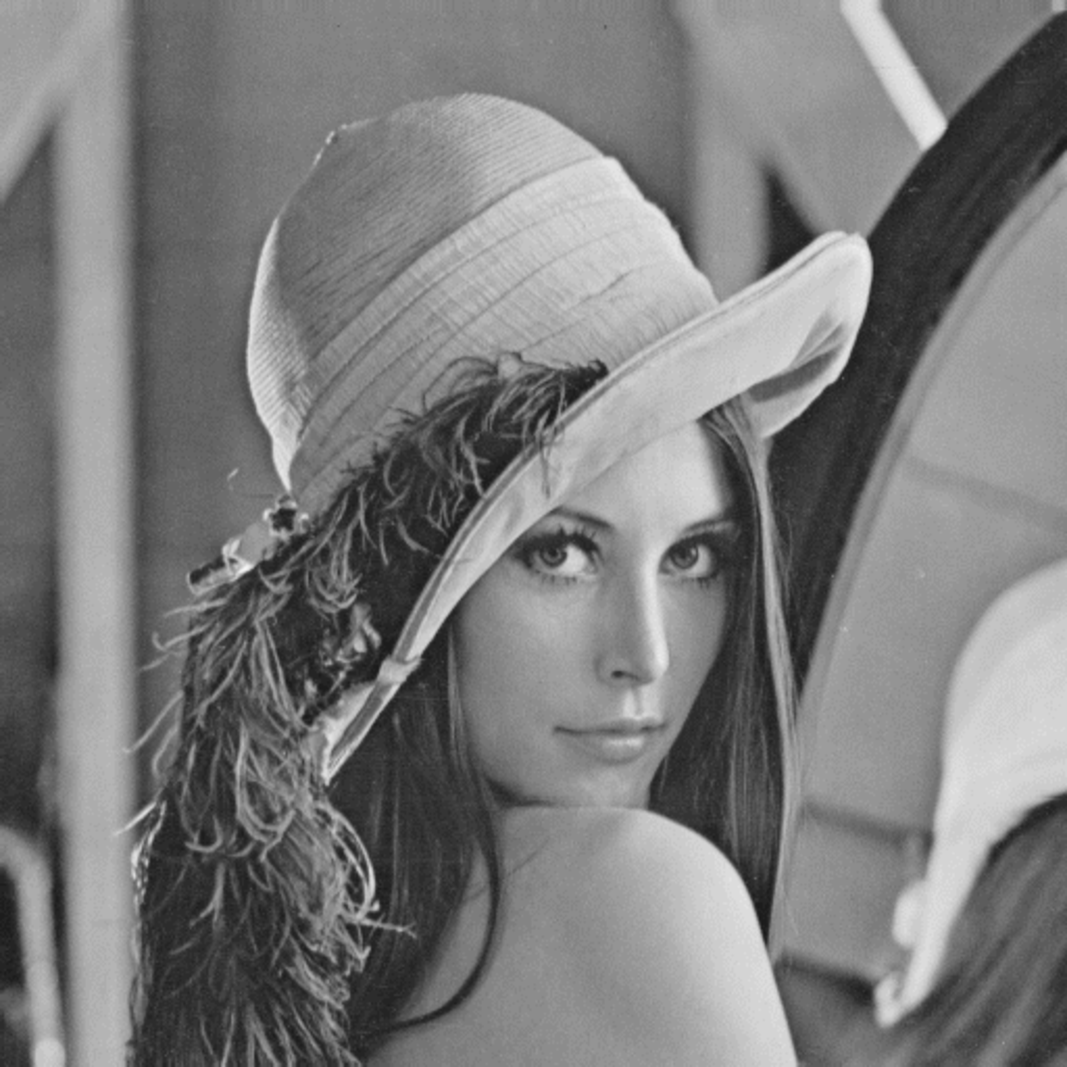
\includegraphics[width=0.49\textwidth]{figures/lena.pdf}
	\caption{Immagine di Lena non compressa}
	\label{fig:lena}
\end{figure}
\columnbreak
\begin{figure}[H]
	\centering
	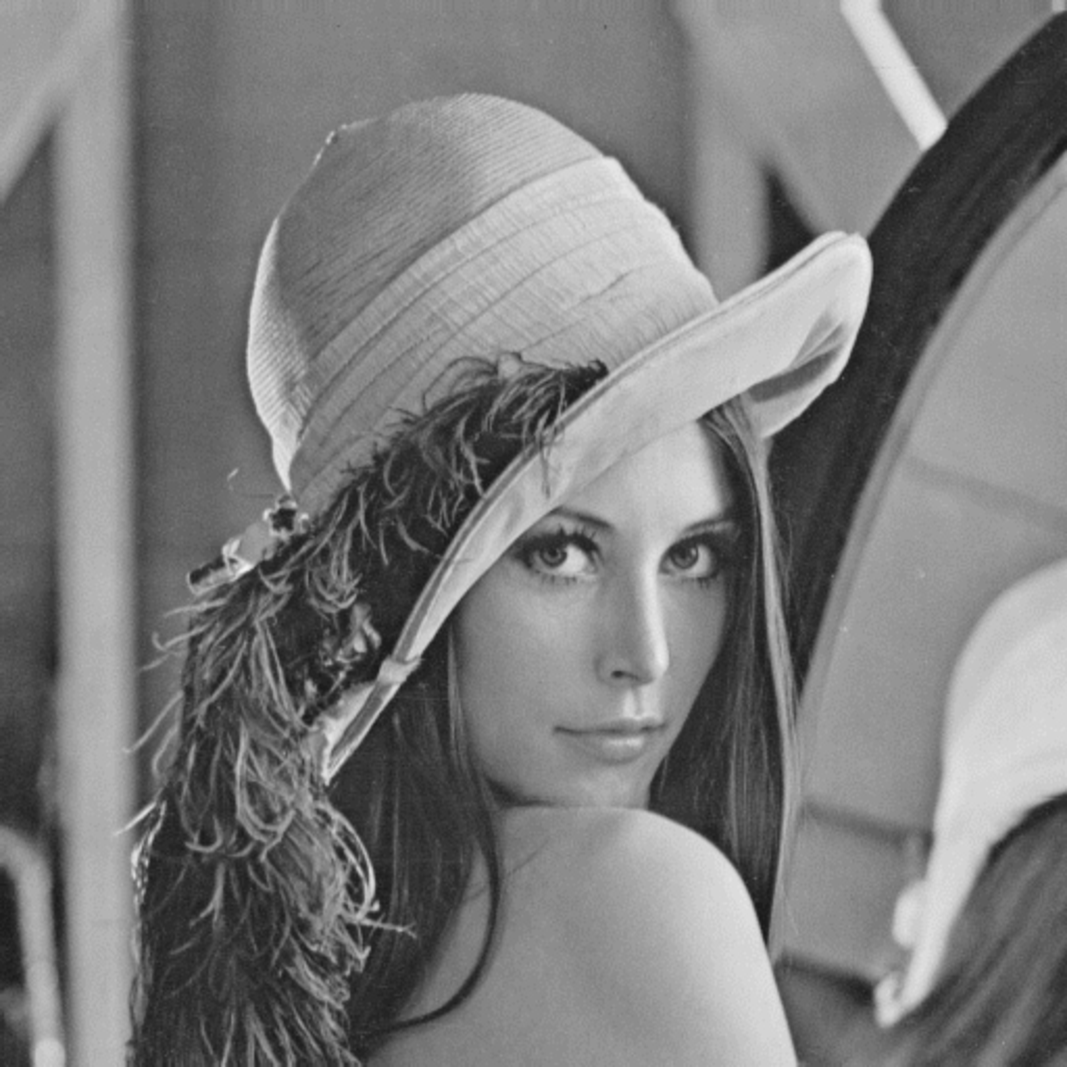
\includegraphics[width=0.49\textwidth]{figures/lena_compressed_f8_d12.pdf}
	\caption{Immagine di Lena compressa con DCT2, con $f=8$ e $d=12$}
	\label{fig:lena_compressed_f8_d12}
\end{figure}
\end{multicols}
\begin{multicols}{2}
\begin{figure}[H]
	\centering
	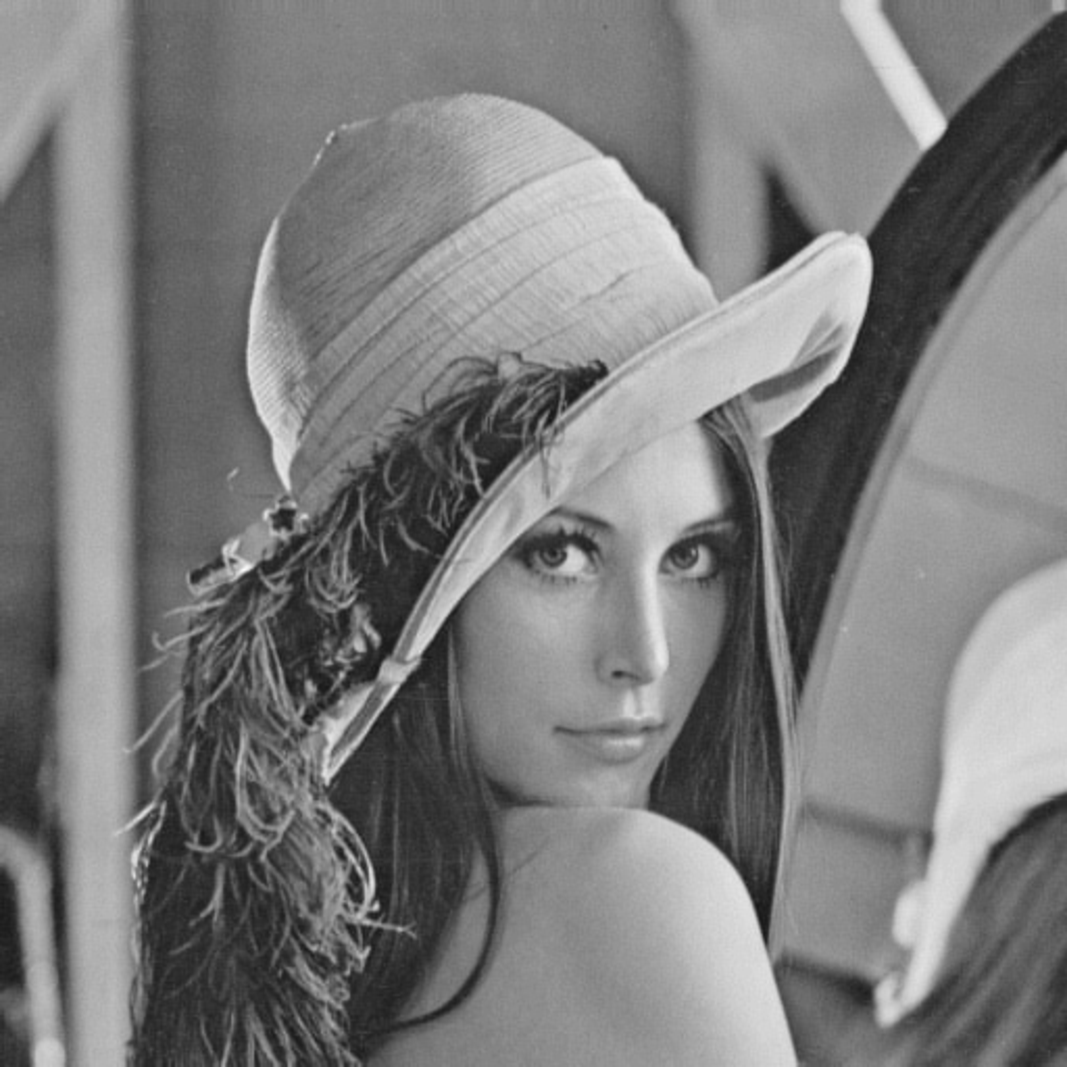
\includegraphics[width=0.5\textwidth]{figures/lena_compressed_f8_d8.pdf}
	\caption{Immagine di Lena compressa con DCT2, con $f=8$ e $d=8$}
	\label{fig:lena_compressed_f8_d8}
\end{figure}
\columnbreak
\begin{figure}[H]
	\centering
	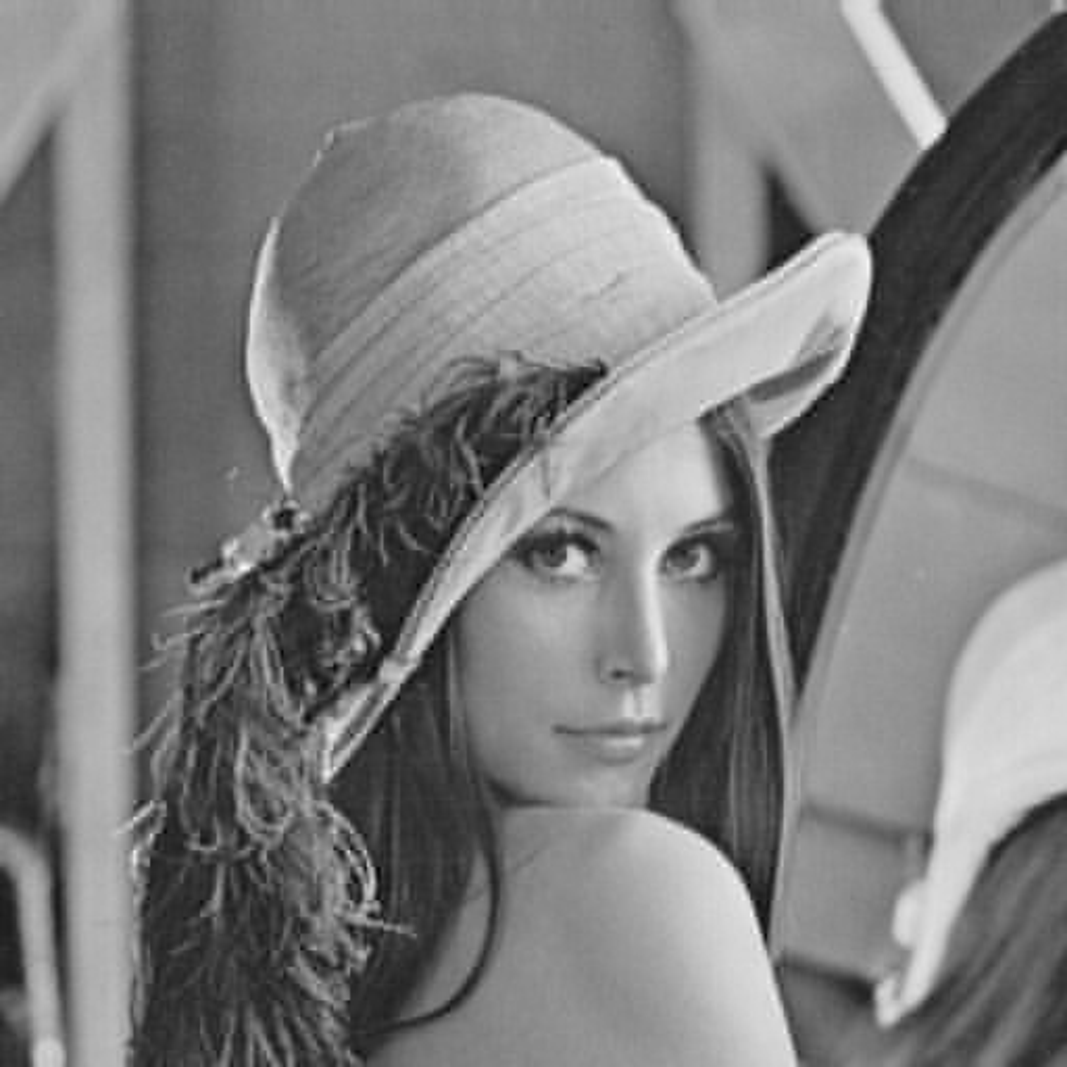
\includegraphics[width=0.5\textwidth]{figures/lena_compressed_f8_d4.pdf}
	\caption{Immagine di Lena compressa con DCT2, con $f=8$ e $d=4$}
	\label{fig:lena_compressed_f8_d4}
\end{figure}
\end{multicols}
\clearpage

\begin{multicols}{2}
	
\begin{figure}[H]
	\centering
	
\includegraphics[width=0.5\textwidth]{figures/lena_compressed_f8_d2.pdf}
	\caption{Immagine di Lena compressa con DCT2, con $f=8$ e $d=2$}
	\label{fig:lena_compressed_f8_d2}
\end{figure}
\columnbreak
\begin{figure}[H]
	\centering
	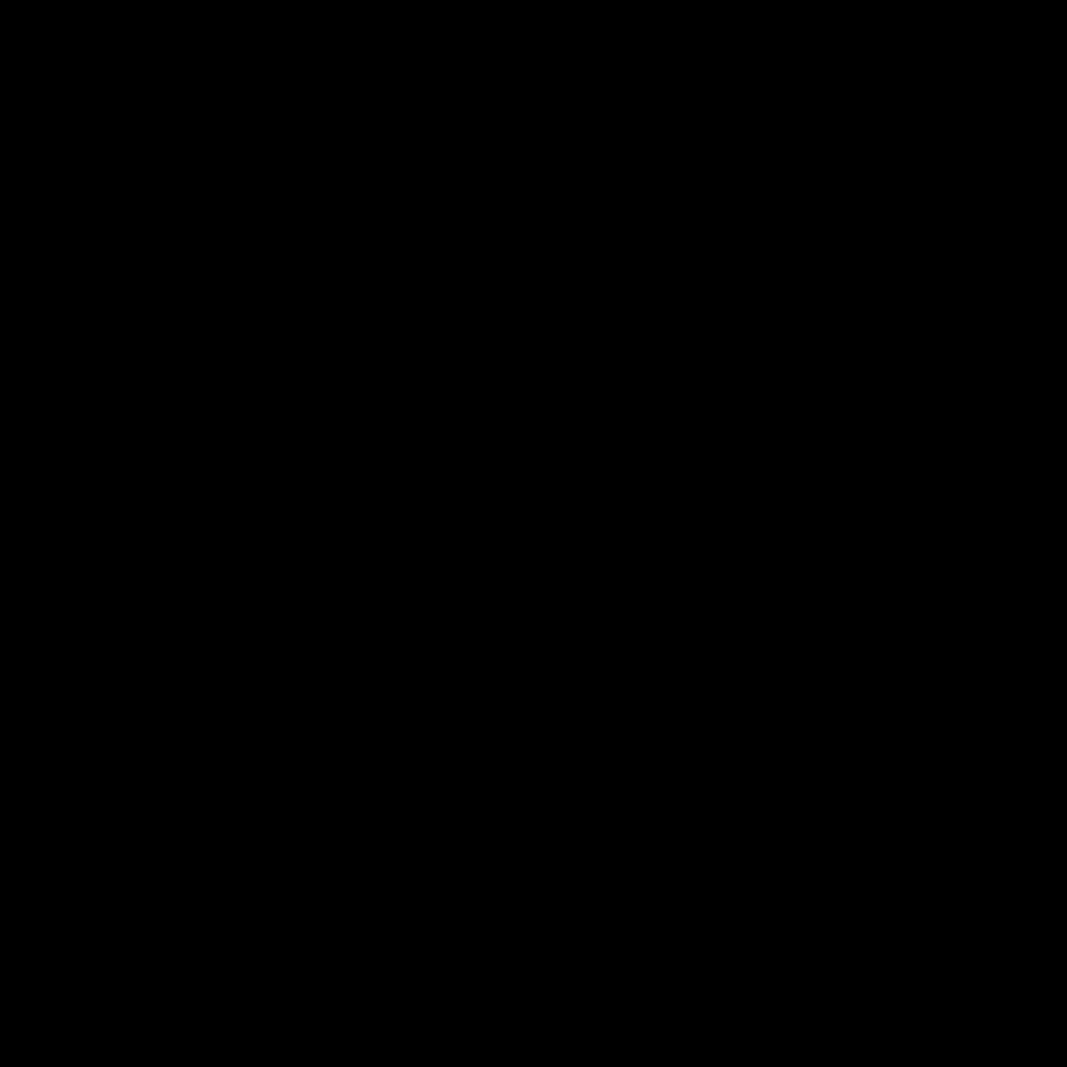
\includegraphics[width=0.5\textwidth]{figures/lena_compressed_f8_d0.pdf}
	\caption{Immagine di Lena compressa con DCT2, con $f=8$ e $d=0$}
	\label{fig:lena_compressed_f8_d0}
\end{figure}
\end{multicols}

    \chapter{Struttura del progetto}
    La struttura del progetto è organizzata in due macro package, il package \texttt{GUI}(Graphical User Interface) si occupa unicamente di gestire 
l'interfaccia utente, mentre il package \texttt{backend} contiene l'implementazione della nostra DCT2, 
la configurazione dei benchmark, la logica per la compressione delle immagini(con la DCT2 nel formato fast
offerta dalla libreria esterna \texttt{JTransform}) e la generazione dei risultati in formato CSV per i 
benchmark e immagini in formato BMP per la compressione delle immagini.
\\
La figura \ref{fig:project_structure} mostra la struttura del progetto. 
\begin{figure}[hbt]
    \centering
    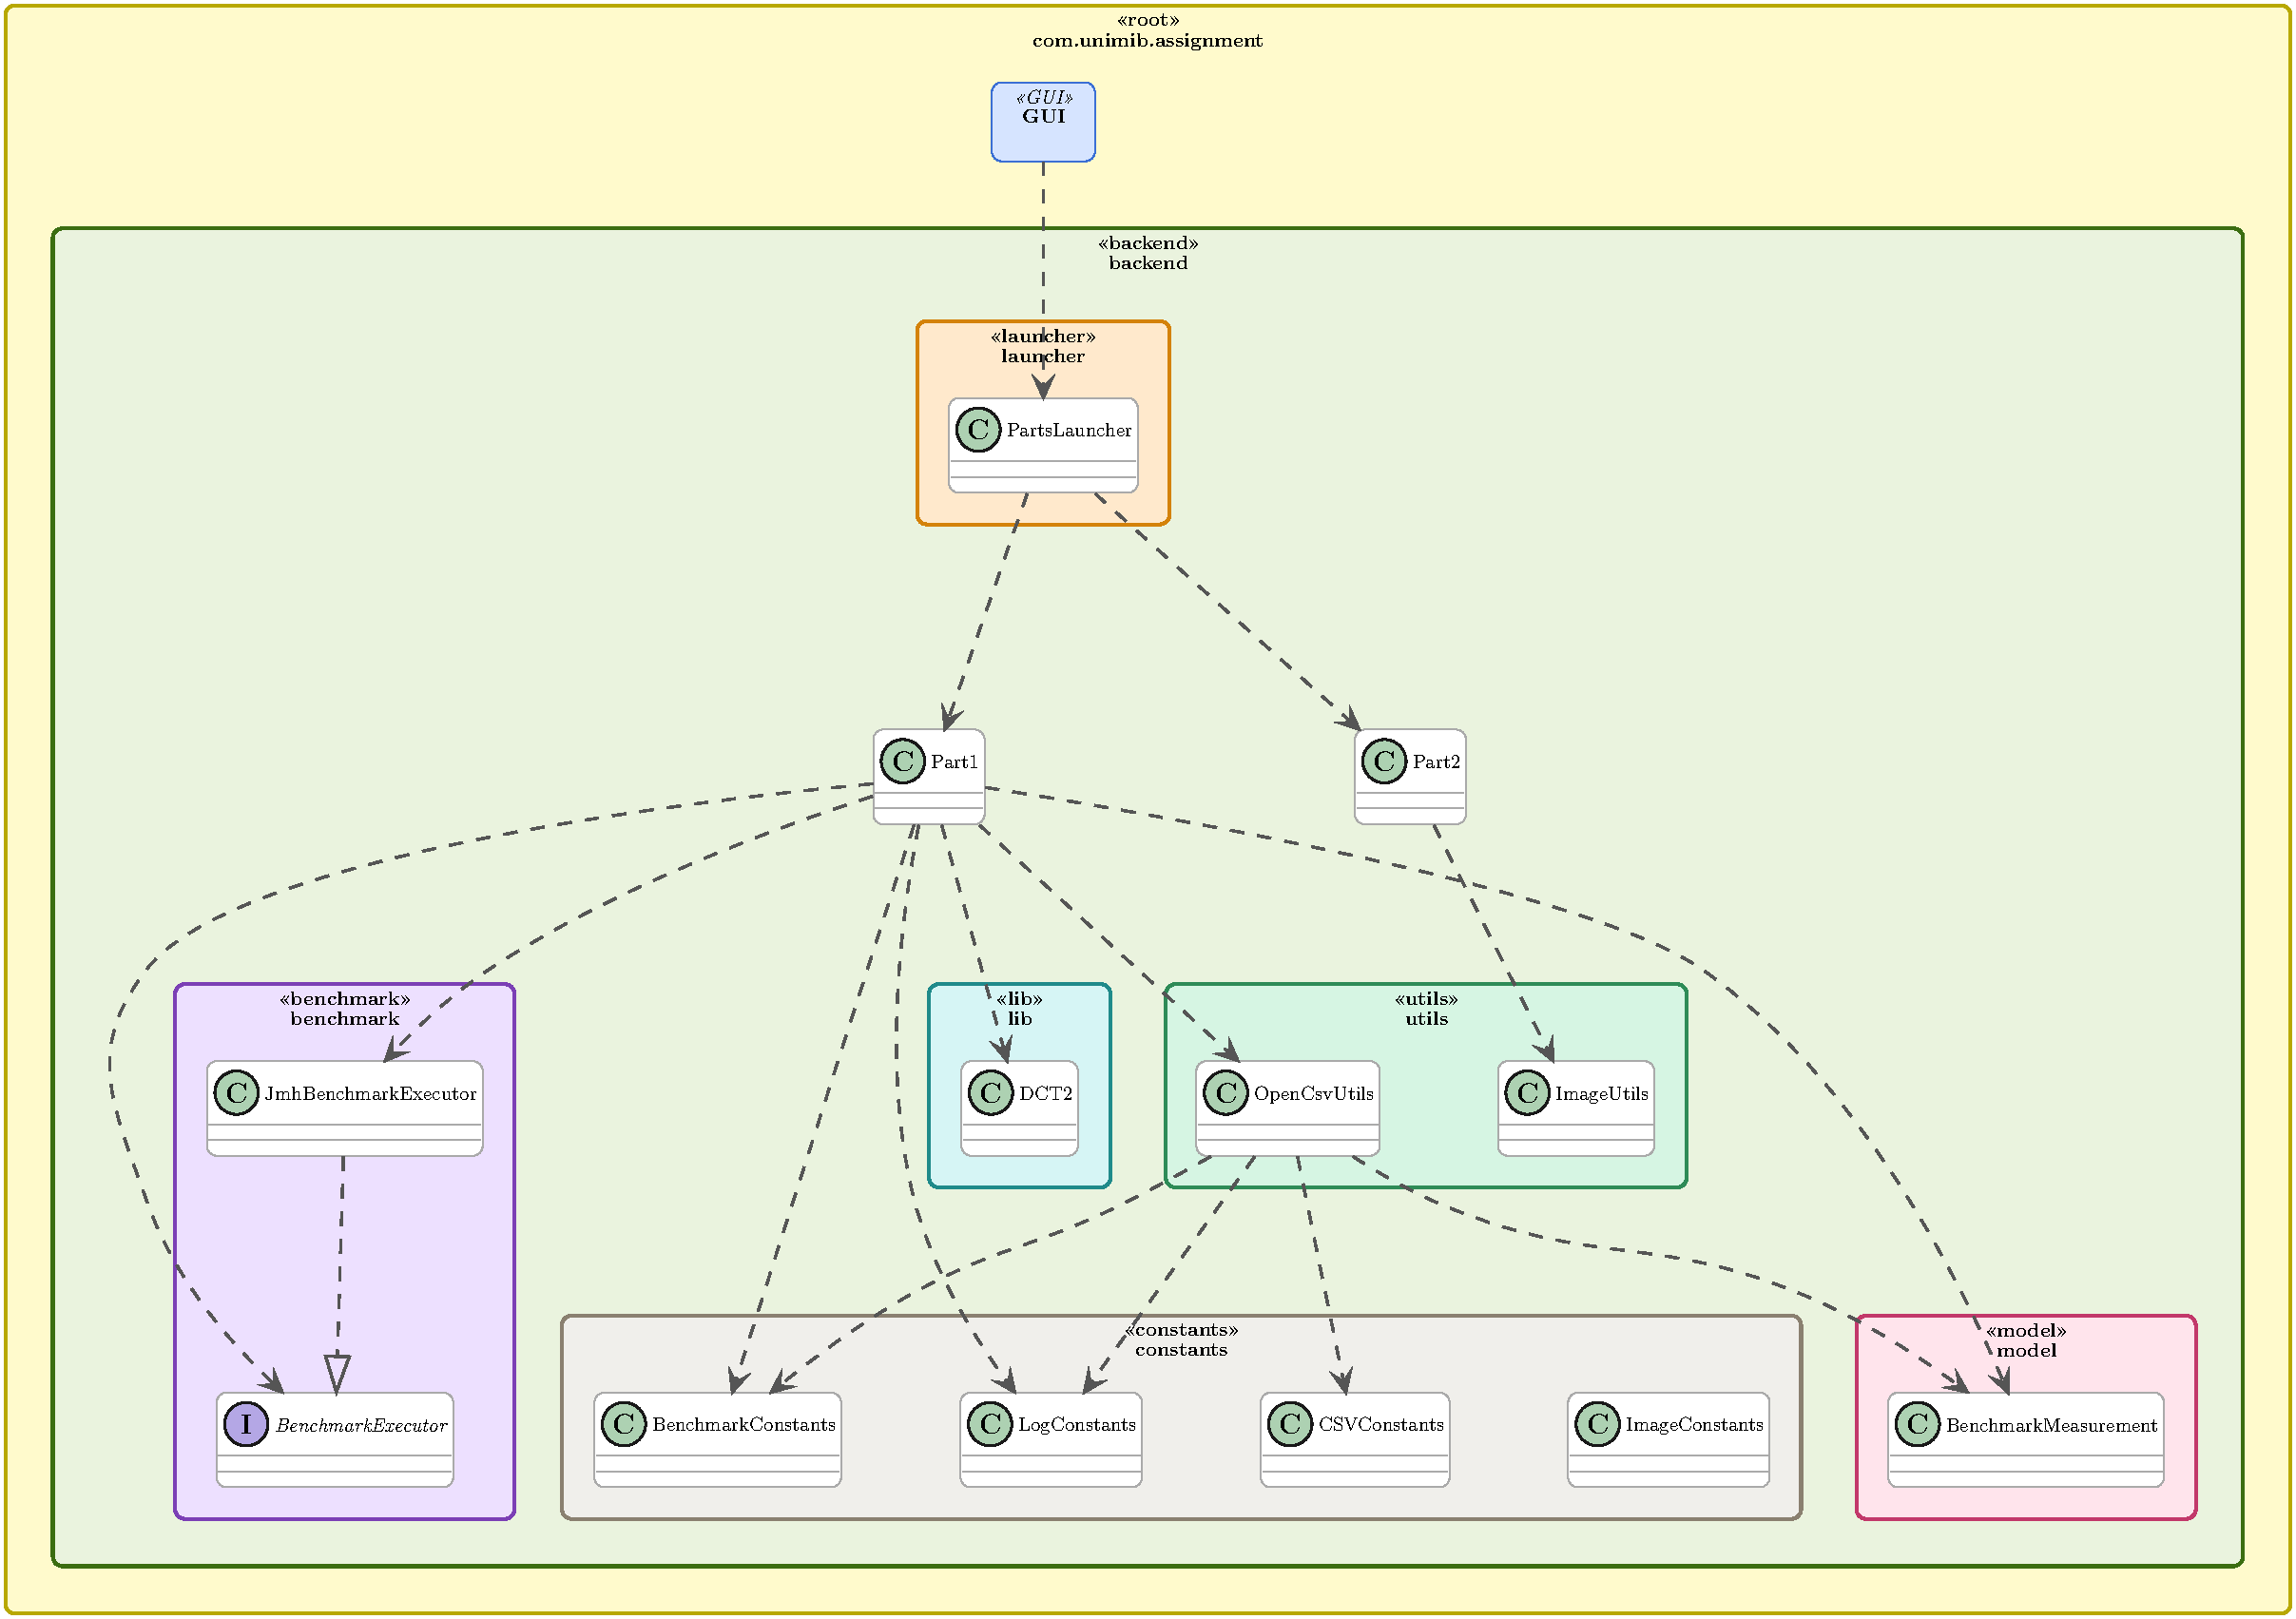
\includegraphics[width=\textwidth]{../architecture/architecture.pdf}
    \caption{Struttura del progetto}
    \label{fig:project_structure}
\end{figure}
\clearpage
\section{Implementazione della DCT2}
Il package \texttt{com.unimib.assignment.backend.lib} contiene l'implementazione della DCT2, questa classe 
implementa un metodo chiamato DCT-II che funge da algoritmo core per i due metodi offerti: 
\lstinputlisting[
	language=Java,
	style = Java,
	caption = Algoritmo DCTII(DCT2) implementato nel package \texttt{lib},
	firstline=79,
	lastline=107,
	label=ls:DCT2
]{../code/src/main/java/com/unimib/assignment/backend/lib/DCT2.java}
Questa implementazione è utilizzata sia per il metodo forward(DCT2):
 \lstinputlisting[
	language=Java,
	style = Java,
	caption = Algoritmo forward implementato nel package \texttt{lib},
	firstline=38,
	lastline=44,
	label=ls:DCT2
]{../code/src/main/java/com/unimib/assignment/backend/lib/DCT2.java}
che per il metodo inverse(IDCT2): 
\lstinputlisting[
	language=Java,
	style = Java,
	caption = Algoritmo inverse implementato nel package \texttt{lib},
	firstline=57,
	lastline=64,
	label=ls:DCT2
]{../code/src/main/java/com/unimib/assignment/backend/lib/DCT2.java}
Questo approccio ci permette di avere un codice più pulito e leggibile, 
evitando la duplicazione del codice per i due metodi.
\footnote{L'implementazione della DCT2 si appoggia alla libreria EJML, questo permette di avere
un codice più leggibile rispetto a un'implementazione basata su matrici}

\section{Part1 e Part2}

Il package \texttt{com.unimib.assignment.backend.launcher} offre la classe \texttt{PartsLauncher},
che espone alla UI due metodi: \texttt{launchAndHandlePart1}, per l'avvio dei benchmark, e
\texttt{launchPart2}, per la compressione delle immagini.

\paragraph{launchAndHandlePart1}
si occupa di invocare la classe \texttt{Part1}, responsabile della gestione del processo di esecuzione dei 
benchmark e della memorizzazione dei risultati.

Come prima operazione, richiama il metodo \texttt{randomMatrix} per generare le matrici casuali da utilizzare
nei benchmark. Tali matrici vengono create prima dell'esecuzione dei test e condivise tra il benchmark 
della nostra implementazione della DCT2 e quello della libreria, così da garantire risultati confrontabili. 
Le dimensioni delle matrici sono memorizzate nell'array di interi \texttt{BENCHMARK\_BLOCK\_SIZES}.

Per l'esecuzione dei benchmark, la classe \texttt{Part1} si occupa di:
\begin{enumerate}
\item invocare la classe \texttt{JmhBenchmarkExecutor}, responsabile della configurazione e dell'esecuzione 
dei benchmark tramite JMH. Tale classe gestisce le iterazioni di warmup 
(\texttt{DEFAULT\_WARMUP\_ITERATIONS} = 3) e quelle di misurazione 
(\texttt{DEFAULT\_MEASUREMENT\_ITERATIONS} = 5), salvando i risultati nel record 
\textsl{BenchmarkMeasurement(size, meanTimeMine, meanTimeLib)}. I tempi sono memorizzati in secondi;
\item salvare i risultati contenuti nel record \textsl{BenchmarkMeasurement} in un file CSV utilizzando la c
lasse \texttt{OpenCsvUtils}, che si appoggia alla libreria opensource \texttt{OpenCSV} \cite{opencsv};
\item gestire eventuali richieste di terminazione forzata del benchmark provenienti dalla UI, 
interrompendone l'esecuzione.
\end{enumerate}

\paragraph{launchPart2}
Si occupa di eseguire la compressione delle immagini utilizzando la trasformata DCT2 fornita dalla libreria
\texttt{JTransform}, di inviare l'immagine compressa alla UI e di salvare le immagini compresse in formato BMP.

La classe \texttt{Part2} contiene i seguenti metodi:

\begin{itemize}
    \item \texttt{BufferedImage compress(Pair<String, BufferedImage> imageInfo, int F, int d)}: esegue l'intera pipeline di compressione dell'immagine:
    \begin{enumerate}
        \item converte l'immagine di input in una matrice di \texttt{double};
        \item ritaglia la matrice in modo che le sue dimensioni siano multipli di \texttt{F};
        \item per ogni blocco di dimensione \texttt{F} $\times$ \texttt{F}, richiama il metodo \texttt{compressBlock} per effettuare la compressione;
        \item converte la matrice risultante in una \texttt{BufferedImage};
        \item salva l'immagine compressa nella cartella \texttt{output} e successivamente la inoltra alla UI.
    \end{enumerate}

    \item \texttt{void compressBlock(double[][] signal, int i, int j, int F, int d)}: comprime un blocco dell'immagine di dimensione \texttt{F} $\times$ \texttt{F}:
    \begin{enumerate}
        \item copia il blocco in una matrice di \texttt{double};
        \item applica la DCT2 al blocco utilizzando il metodo \texttt{forward(matrix, scale)} dell'oggetto \texttt{DoubleDCT\_2D} della libreria \texttt{JTransform}, impostando \texttt{scale = true}. In questo modo viene utilizzata una normalizzazione ortonormale, coerente con quella adottata nella nostra implementazione della DCT2;
        \item elimina le componenti ad alta frequenza in base al parametro \texttt{d};
        \item applica la trasformata inversa IDCT2 mediante il metodo \texttt{inverse(matrix, scale)}, con \texttt{scale = true};
        \item richiama il metodo \texttt{shiftBlockBy255} per riportare i valori del blocco nell'intervallo \([0, 255]\);
        \item copia il blocco compresso nella matrice dell'immagine risultante.
    \end{enumerate}

    \item \texttt{void shiftBlockBy255(double[][] matrix)}: effettua uno shift dei valori nell'intervallo \([0, 255]\), riportandoli nel dominio delle immagini BMP.
\end{itemize}

I metodi di conversione tra \texttt{BufferedImage} e matrici di \texttt{double} e il salvataggio
in formato BMP sono implementati nella classe \texttt{ImageUtils}.

\subsection{GUI}
Il package \texttt{com.unimib.assignment.GUI} offre 3 schermate principali: due schermate iniziali per il lancio dei benchmark
e per l'avvio della compressione delle immagini, una schermata dedicata alla compressione e una schermata per
l'inserimento dei parametri di compressione. La Figura \ref{fig:main-screen-1} mostra la schermata iniziale per la scelta tra benchmark e compressione,
la Figura \ref{fig:main-screen-2} la schermata iniziale una volta scelta l'opzione benchmark, la Figura \ref{fig:compression-screen}
la schermata di compressione delle immagini e la Figura \ref{fig:parameters-screen} la schermata d'inserimento dei parametri di compressione.
Per l'avvio dei benchmark e della compressione delle immagini, la UI si appoggia alla classe 
\texttt{PartsLauncher} del package \texttt{backend.launcher}.
\begin{figure}[hbt]
    \centering
    \begin{minipage}[t]{0.44\textwidth}
        \centering
        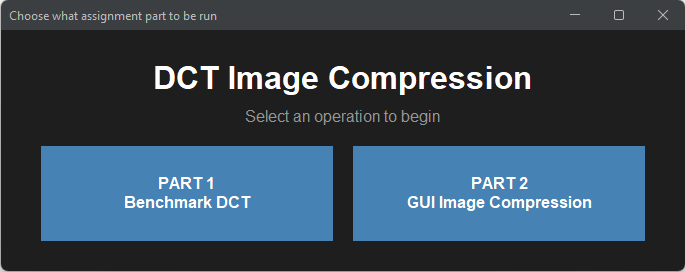
\includegraphics[width=\linewidth]{figures/main-screen-1.png}

        \small Schermata iniziale per la scelta tra benchmark e compressione delle immagini
        \label{fig:main-screen-1}
    \end{minipage}\hfill
    \begin{minipage}[t]{0.44\textwidth}
        \centering
        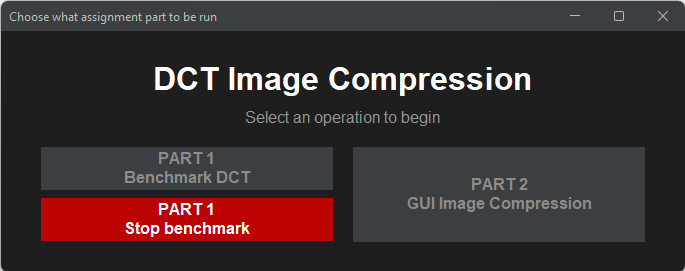
\includegraphics[width=\linewidth]{figures/main-screen-2.png}

        \small Schermata iniziale una volta scelta l'opzione di benchmark
        \label{fig:main-screen-2}
    \end{minipage}
\end{figure}

\begin{figure}[hbt]
    \centering
    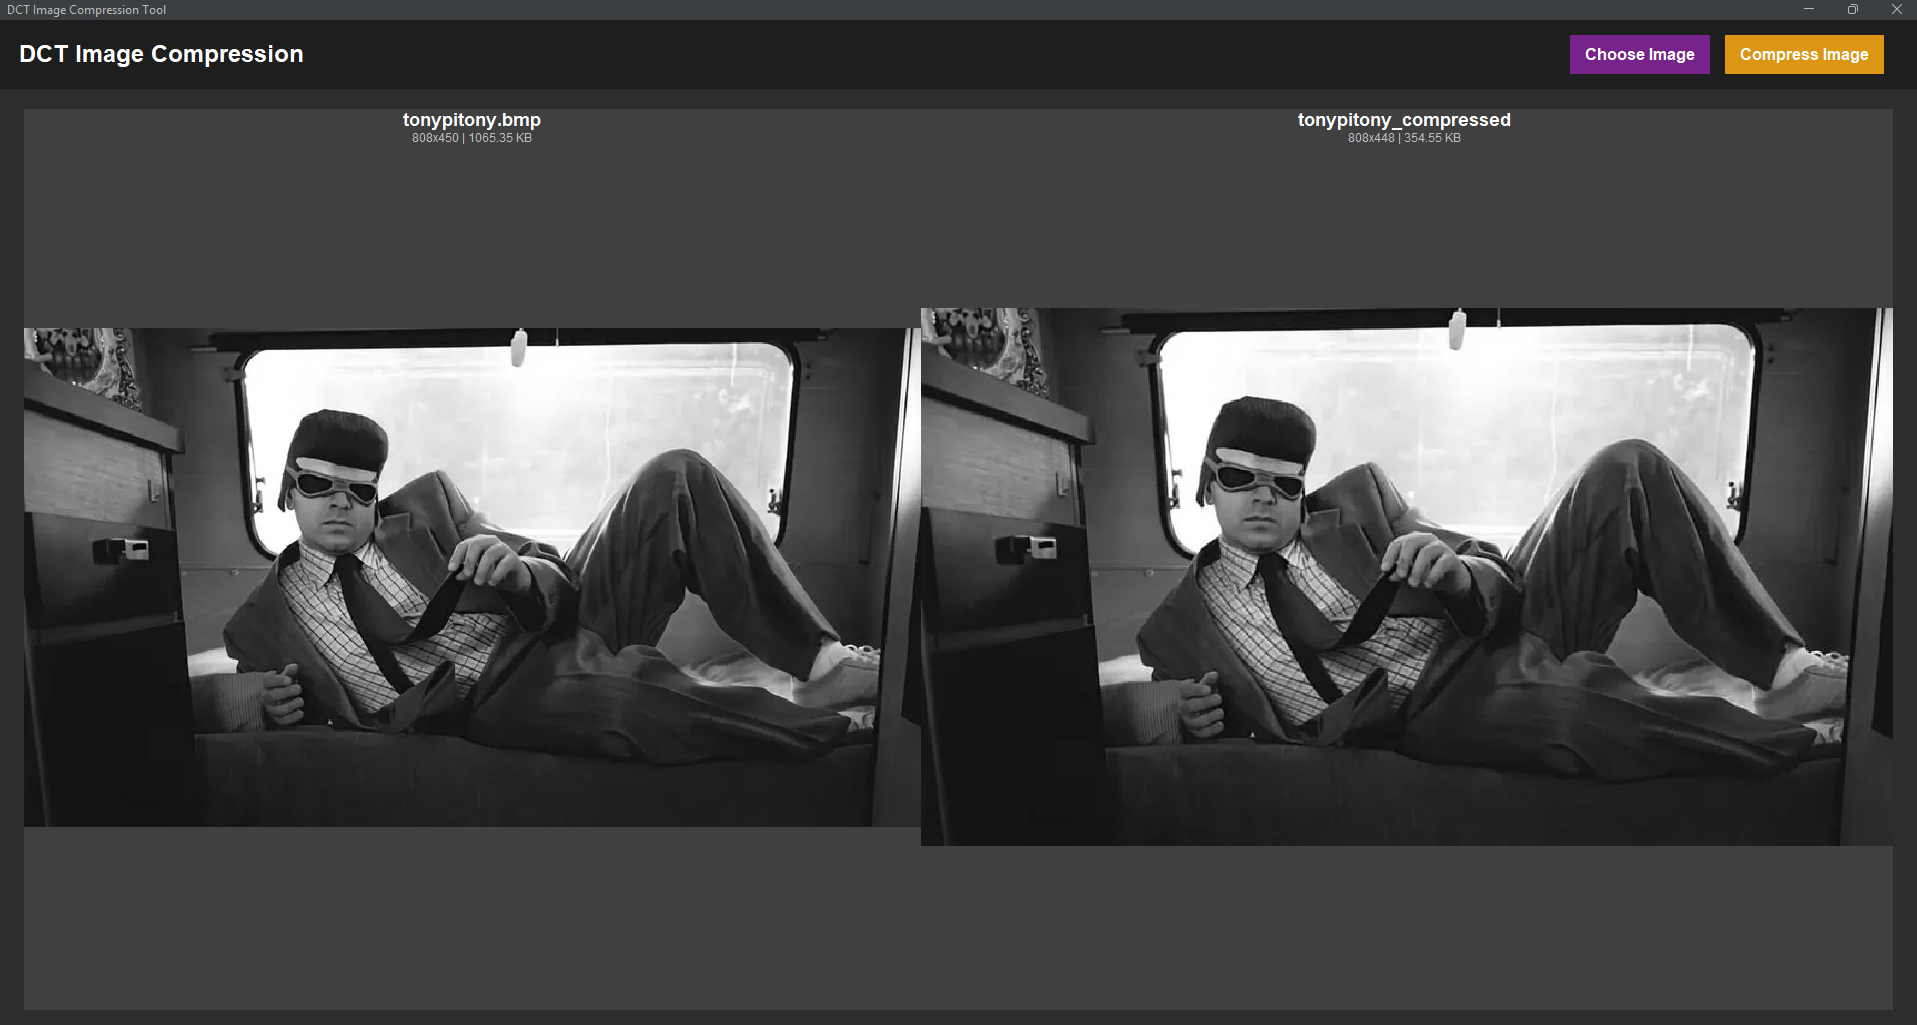
\includegraphics[width=\textwidth]{figures/compression-screen.png}
    \caption{Schermata di compressione delle immagini}
    \label{fig:compression-screen}
\end{figure}

\begin{figure}[hbt]
    \centering
    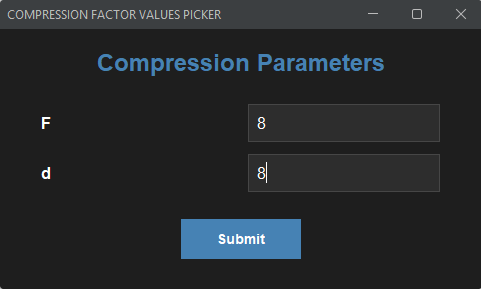
\includegraphics[width=0.35\textwidth]{figures/parameters-screen.png}
    \caption{Schermata d'inserimento dei parametri di compressione}
    \label{fig:parameters-screen}
\end{figure}

    \printbibliography
\end{document}


